\chapter{Matematik}
\label{cha:matematik}

I dette appendiks skal vi indføre nogle nyttige matematiske redskaber,
der er essentielle for fysikken. Selvom du måske kender noget af
matematikken i forvejen, så anbefaler vi alligevel kraftigt, at du
læser appendikset, fordi vi sandsynligvis præsenterer det på en anden
måde, end du er vant til fra gymnasiet.

\section{Polære Koordinater, Cosinus og Sinus}
Forestil dig en lille kugle for enden af en snor, der roterer rundt i
en cirkelbevægelse som på tegningen nedenfor.
\begin{center}
  \begin{tikzpicture}[scale=.8]
    \draw [->] (-3.2,0) -- (3.2,0);
    \draw [->] (0,-3.2) -- (0,3.2);
    \draw (0,0) circle (2.4);
    \draw (0,0) -- (1.49186,1.87998);
    \draw [fill] (1.49186,1.87998) circle (.07);
    \draw [dashed] (1.49186,1.87998) -- (1.49186,0);
    \draw [dashed] (1.49186,1.87998) -- (0,1.87998);
    \node [right] at (3.2,0) {$x$};
    \node [above] at (0,3.2) {$y$};
    \node at (1.17*1.49186,1.17*1.87998) {$P$};
    \node [below] at (1.49186,0) {$x$};
    \node [left] at (0,1.87998) {$y$};
    \draw [->] (1.2*.4,0) to[out=70, in=-25] (1.2*.2486,1.2*.3133);
    \node at (.7,.4) {$\theta$};
    \node [above,rotate=51] at (.5*1.49186,.5*1.87998) {$r$};
    \node [right] at (3,2.5) {$x = r \cos\theta$};
    \node [right] at (3,1.8) {$y = r \sin\theta$};
  \end{tikzpicture}
\end{center}
Kulgen roterer rundt i et to-dimensionelt plan. Lad os sige, at til et
bestemt tidspunkt befinder kulgen sig i punktet $P$. Når vi har lagt
et koordinatsystem som på tegningen kan vi beskrive punket $P$ ved at
angive dets $x$-værdi og $y$-værdi. Disse koordinater ($x$ og $y$)
kaldes \emph{kartesiske} koordinater. Det er muligt at beskrive $P$
ved hjælp af andre koordinater, fx er det i dette tilfælde smart at
beskrive $P$ ved at angive afstanden $r$ fra centrum (origo) og
vinklen $\theta$ mellem $x$-aksen og linjen fra origo til $P$, se
tegningen. Disse koordinater ($r$ og $\theta$) kaldes \emph{polære}
koordinater.

Fordelen ved polære koordinater er tydelig, når vi tænker
på en kulge i en snor, der roterer rundt: Til et senere tidspunkt har
kuglen flyttet sig til et andet punkt på cirklen. I kartesiske
koordinater vil det nye punkt have både en ny $x$- og $y$-værdi, men i
polære koordinater vil vinklen $\theta$ være ny, men radius $r$ er
uændret. Så i polære koordinater er det altså kun én koordinat, der
ændres, når kuglen roterer rundt, hvilket er nemmere at arbejde med en
to, der ændrer sig.

Relationerne mellem kartesiske og polære koordinater er:
\begin{align*} \label{eq:kartesisk/polaer}
  x &= r \cos \theta \\
  y &= r \sin \theta \\
  r &= \sqrt{x^2 + y^2} \\
  \theta &= \arctan (y/x) \; ,
\end{align*}
hvor $\arctan$ er den inverse funktion til tangens, men udtrykket for
$\theta$ vil I ikke få brug for. I udtrykkene for $x$ og $y$ indgår
henholdsvis funktionerne cosinus og sinus. Hvis du ikke kender disse
funktioner, kan du selv finde litteratur om dem, men faktisk er de
defineret som på tegningen: Hvis $\theta$ angiver vinklen mellem
$x$-aksen og et punkt, så er
\begin{align*}
  &\cos \theta = \text{$x$-koordinaten for punktet på cirklen med
    radius $1$}\\
  &\sin \theta = \text{$y$-koordinaten for punktet på cirklen med
    radius $1$}
\end{align*}
Cosinus og sinus har også noget med trekanter at gøre. Hvis vi kigger
på tegningen af cirklen igen, ser vi, at den indeholder to retvinklede
trekanter: $OxP$ og $OyP$, hvor $O$ betegner centrum. I de to
trekanter er hypotenusen $r$, og de to sidelænger er $x = r
\cos\theta$ og $y = r \cos\theta$. Vi kan altså lave følgende tegning,
der illustrerer længderne i en retvinklet trekant:
\begin{center}
  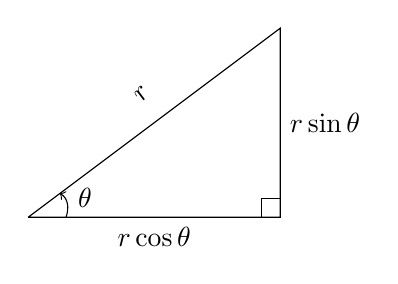
\begin{tikzpicture}[scale=.8]
    \draw [-] (0,0) -- (4,0) -- (4,3) -- (0,0);
    \draw [->] (.6,0) to[out=70, in=-30] (.5,.38);
    \node at (.9,.3) {$\theta$};
    \node [above,rotate=51] at (2,1.8) {$r$};
    \node [below] at (2,0) {$r \cos\theta$};
    \node [right] at (4,1.5) {$r \sin\theta$};
    \draw [-] (3.7,0) -- (3.7,.3) -- (4,.3);
  \end{tikzpicture}
\end{center}
Heraf følger at cosinus og sinus er forholdet mellem to længder i den
retvinklede trekant:
\begin{align*}
  &\cos \theta = \frac{\text{hosliggende side}}{\text{hypotenusen}}\\
  &\sin \theta = \frac{\text{modstående side}}{\text{hypotenusen}}
\end{align*}
Vi definerer også en funktion kaldet tangens:
\[
  \tan \theta = \frac{\sin\theta}{\cos\theta}
  = \frac{\text{modstående side}}{\text{hosliggende side}}
\]
Hvis vi sætter $r=1$ får vi fra Pythagoras' sætning at
\begin{equation*}
  \cos^2 \theta + \sin^2 \theta = 1 \; ,
\end{equation*}
hvor vi har brugt notationen $\cos^2 \theta = (\cos\theta)^2$ og
$\sin^2 \theta = (\sin\theta)^2$.

\section{Differentialregning}
En bil kører på vejen, og den position betegnes $x$. Fordi bilen
bevæger sig, ændrer den position sig med tiden. Hvis vi lader $t$
betegne tiden, så er bilens position en \emph{funktion} af tiden, og
vi skriver $x(t)$. Vi siger også, at $x$ \emph{afhænger} af $t$. Nogle
gange er vi dovne og nøjes med at skrive $x$ i stedet for $x(t)$, men
vi husker på, at $x$ er en funktion af $t$. Måske er vi interesseret i
bilens hastighed $v$, hvilket er ændringen i position pr. ændringen i
tid. Hvis bilens position ændrer sig meget i løbet af kort tid, så er
bilens hastighed stor. Med andre ord er hastigheden til et bestemt
tidspunkt $t$ altså givet som hældningen af grafen for $x(t)$, og
hastigheden er altså selv en funktion af tiden, $v(t)$. Nedenfor ses
et eksempel, hvor bilen kører baglens for $t<5$ s, standser i $t=5$ s,
og kører fremad for $t>5$ s, hvorefter den kører hurtigere og
hurtigere som $v(t)$ vokser.

\begin{center}
  \begin{tikzpicture}
    \begin{scope}[shift={(0,0)}]
      \draw [->] (-.1,0) -- (3.3,0);
      \node [right] at (3.3,0) {$t$};
      \draw [->] (0,-.1) -- (0,2.5);
      \node [above] at (0,2.5) {$x(t)$};
      \draw [blue, domain=-.3:3.3, samples=100]
      % plot (\x, {.8+1.1*cos((\x + .56) r)*cos((3*\x) r)});
      plot (\x, {1/2*\x^2 - \x + 1/3});
      \node [left] at (-.1,0) {$0$};
      \draw (-.1,2) -- (.1,2);
      \node [left] at (-.1,2) {$2$ m};
      \node [below] at (0,-.1) {$0$};
      \draw (2,-.1) -- (2,.1);
      \node [below] at (2,-.1) {$10$ s};
    \end{scope}
    % 
    \begin{scope}[shift={(6,0)}]
      \draw [->] (-.1,0) -- (3.3,0);
      \node [right] at (3.3,0) {$t$};
      \draw [->] (0,-.1) -- (0,2.5);
      \node [above] at (0,2.5) {$v(t)$};
      \draw [blue, domain=-.3:3.3, samples=100]
      % plot (\x, {.8+1.1*cos((\x + .56) r)*cos((3*\x) r)});
      plot (\x, {\x - 1});
      \node [left] at (-.1,0) {$0$};
      \draw (-.1,2) -- (.1,2);
      \node [left] at (-.1,2) {$2$ m/s};
      \node [below] at (0,-.1) {$0$};
      \draw (2,-.1) -- (2,.1);
      \node [below] at (2,-.1) {$10$ s};
    \end{scope}
  \end{tikzpicture}
\end{center}

\subsection{Notation for Differentialkvotienter}
Differentialregning går ud på at beregne hældningen af en graf. Som
allerede illustreret med den kørende bil, så er dette yderst relevant
i fysik. En stor del af fysik har at gøre med hvordan noget ændrer
sig, når man ændrer et eller andet, f.eks. hvordan positionen ændrer
sig, når tiden ændrer sig. Tit afhænger fysiske størrelser af mere end
én variabel, og derfor betragter vi generelt funktioner af flere
variable,
\[
f(x,y,z,\dots) \; .
\]
Hvis vi vil finde hældningen skal vi specificere hældningen
mht. hvilken variabel. Hvis vi vil finde hældningen mht. $x$, må vi
holde $y, z, \dots$ fast og kun ændre $x$. Da kan vi tegne grafen for
$f$ som funktion af $x$ og finde hældningen. Hældningen for $f$
mht. $x$ betegnes
\begin{align*}
  \dl{f(x,y,z\dots)}{x}
  \qquad
  \text{eller}
  \qquad
  \dl{f}{x}
  \qquad
  \text{eller blot}
  \qquad
  \d{f}{x} \; ,
\end{align*}
og $\d{f}{x}$ er en funktion af $x$ (og de øvrige variable
$y,z\dots$), der kaldes \emph{differentialkvotienten} (eller \emph{den
  afledte}) af $f$ mht. $x$. Når vi beregner differentialkvotienten
siger vi, at vi \emph{differentierer} (eller \emph{afleder})
funktionen $f$ mht. $x$. Du har måske allerede stødt på dette, men
brugt mærke-notationen i stedet:
\begin{align*}
  \d{f}{x} = f'(x) \; .
\end{align*}
Mærke-notationen $f'(x)$ er uheldig, fordi den kun kan anvendes for
funktioner af én variabel; hvis funktionen afhænger af to variable,
hvilken én heviser mærket så til? Da $\d{f}{x}$ også er en funktion,
kan vi differentiere den igen, enten mht. $x$ igen eller en af de
andre variable, hvilket skrives
\begin{align*}
  \dl{\left(\d{f}{x}\right)}{x}
  = \dl{\d{f}{x}}{x}
  = \dd{f}{x}
  \qquad
  \text{og}
  \qquad
  \dl{\left(\d{f}{x}\right)}{y} = \dl{\d{f}{x}}{y} \; .
\end{align*}
I det særlige tilfælde, hvor vi differentierer en funktion mht. tiden
$t$, så bruger vi tit en særlig prik-notation:
\begin{align*}
  \d{f}{t} = \dt{f}
  \qquad
  \text{og}
  \qquad
  \dl{\d{f}{t}}{t} = \dd{f}{t} = \ddt{f} \; .
\end{align*}
\textsl{Sidebemærkning:} Hvis man vil, kan man tænke på $\d{}{x}$ som
en operator, der opererer på funktionen $f$. Når vi ganger operatoren
$\d{}{x}$ på $f$ fra venstre, vil dens operation være at finde
hældningen af $f$ mht. $x$. I sig selv giver $\d{}{x}$ ikke så meget
mening, men når den får lov til at operere på en funktion $f$, så får
vi en ny funktion, $\d{f}{x}$.

\subsection{Regneregler}
Vi skal ikke gå i detaljer med, hvordan man matematisk finder
differentialkvotienter. Derimod vil vi postulere en række regneregler,
og dem skal vi bruge til at regne differentialkvotienten ud for en
masse funktioner. Nedenfor er $f$ og $g$ to funktioner af $x$ og
evt. flere variable, $f(x,\dots)$ og $g(x,\dots)$, og $a$ er en
konstant (dvs. afhænger ikke af $x$).

\begin{enumerate}
\item\label{itm:d-skalering} \textbf{Konstant skalering.}\\
  Hvis $a$ er en konstant kan den trækkes udenfor differentiationen.
  \[
  \dl{(a f)}{x} = a \, \d{f}{x} \; .
  \]
\item\label{itm:d-sum} \textbf{Sum.}\\
  En sum differentieres ved at differentere hvert led.
  \[
  \dl{(f+g)}{x} = \d{f}{x} + \d{g}{x} \; .
  \]
\item\label{itm:d-produkt} \textbf{Produkt.}\\
  Et produkt differentieres ved skiftevis differentiere hver faktor.
  \[
  \dl{(f \cdot g)}{x} =
  \left(\d{f}{x}\right) \cdot g + f \cdot \left(\d{g}{x}\right) \; .
  \]
\item\label{itm:d-kvotient} \textbf{Kvotient.}\\
  En kvotient differentieres på følgende vis.
  \[
  \dl{\left( \frac{f}{g} \right)}{x}
  = \frac{\left(\d{f}{x}\right)
    \cdot g - f \cdot \left(\d{g}{x}\right)}{g^2} \; .
  \]
\item\label{itm:d-kaederegel} \textbf{Kædereglen.}\\
  En sammensat funktion, $f(g(x))$, differentieres ved at
  differentiere den indre funktion, $g(x)$, mht. $x$ og gange med den
  ydre funktion $f(g)$ differentieret mht. den indre funktion, $g$.
  \[
  \dl{f(g(x))}{x} = \d{g}{x} \cdot \d{f}{g} \; .
  \]
\item\label{itm:d-kommutation} \textbf{Ombytning af rækkefølgen.}\\
  Hvis man differentierer en funktion mht. to forskellige variable, må
  man ombytte rækkefølgen af differentiationen.
  \[
  \dl{\d{f}{x}}{y} = \dl{\d{f}{y}}{x}
  \]
\end{enumerate}

Med de ovenstående regler kan differentialkvotienten af enhver
funktion simplificeres, så den kan beregnes ved at kende
differentialkvotienten af nogle simplere funktioner. Nu giver vi en
liste over differentialkvotienter for en række simple funktioner.

\begin{enumerate}[resume]
\item\label{itm:d-konstant} \textbf{Konstant.}\\
  \[
  \dl{a}{x} = 0 \; .
  \]
\item\label{itm:d-potens} \textbf{Potensfunktion.}\\
  \[
  \dl{x^a}{x} = a x^{a-1} \; .
  \]
  Specielt gælder der
  \begin{align*}
    &\dl{x}{x} = 1 &&(a=1)\\
    &\dl{x^2}{x} = 2 x &&(a=2)\\
    &\dl{x^3}{x} = 3 x^2 &&(a=3)\\
    &\dl{\sqrt{x}}{x} = \frac{1}{2\sqrt{x}} &&(a=\tfrac{1}{2})\\
    &\dl{\frac{1}{x}}{x} = - \frac{1}{x^2} &&(a=-1)\\
    &\dl{\frac{1}{x^2}}{x} = - \frac{2}{x^3} &&(a=-2)
  \end{align*}
  Kombineret med regel 1 og 2, får man for polynomier
  \[
  \dl{(a_0 + a_1 x + a_2 x^2 + a_3 x^3 + \dots + a_n x^n)}{x}
  = a_1 + 2a_2 x + 3a_3 x^2 + \dots + na_n x^{n-1}
  \]
  Specielt for en lineær funktion og en parabel har vi
  \begin{align*}
    &\dl{ (a_0 + a_1 x) }{x} = a_1 && (n=1)\\
    &\dl{ (a_0 + a_1 x + a_2 x^2) }{x} = a_1 + 2a_2 x && (n=2)
  \end{align*}
\item\label{itm:d-exp} \textbf{Eksponentialfunktion.}\\
  \[
  \dl{e^x}{x} = e^x \; .
  \]
\item\label{itm:d-ln} \textbf{Naturlig logaritme.}\\
  \[
  \dl{\ln x}{x} = \frac{1}{x} \; .
  \]
\item\label{itm:d-sin} \textbf{Sinus.}\\
  \[
  \dl{\sin x}{x} = \cos x \; .
  \]
\item\label{itm:d-cos} \textbf{Cosinus.}\\
  \[
  \dl{\cos x}{x} = - \sin x \; .
  \]
\end{enumerate}

\subsection{Eksempel 1}
Vi vil differentiere funktionen $F(x) = (3 - x^2) e^{-x^2}$
mht. $x$. Vi starter med at betragte $F(x)$ som et produkt af to
funktioner, $3-x^2$ og $e^{-x^2}$, og bruger derfor regel 3.
\[
\d{F}{x} =
\left(\dl{(3-x^2)}{x}\right) \cdot e^{-x^2}
+ (3-x^2) \cdot \left(\dl{e^{-x^2}}{x}\right)
\]
Fra regel 8 for en parabel med $a_0 = 3$, $a_1 = 0$ og $a_2 = -1$ har vi, at
\[
\dl{(3-x^2)}{x} = -2x \; .
\]
Dernæst vil vi differentiere $e^{-x^2}$, som vi betragter som en
sammensat funktion. Regel 5 med $g(x) = -x^2$ og $f(g(x)) = e^{g(x)}$
giver, at
\[
\dl{e^{-x^2}}{x} = \dl{(-x^2)}{x} \cdot \dl{e^g}{g}
= -2x \cdot e^g
= -2x e^{-x^2} \; .
\]
Vi kan nu samle resultaterne og beregne
\[
\d{F}{x} = (-2x) \cdot e^{-x^2} + (3-x^2) \cdot (-2x e^{-x^2})
= -2x(4 - x^2) e^{-x^2} \; .
\]

\begin{figure}[htbp]
  \centering
  \begin{tikzpicture}
    \begin{scope}[shift={(0,0)}]
      \draw [->] (-3,0) -- (3,0);
      \node [right] at (3,0) {$x$};
      \draw [->] (0,-.1) -- (0,3.3);
      \node [above] at (0,3.3) {$F(x)$};
      \draw [blue, domain=-3:3, samples=300]
      plot (\x, {(3-\x*\x)*exp(-\x*\x)});
      \draw (-.1,1) -- (.1,1);
      \node [left] at (-.1,1) {$1$};
      \node [below] at (0,-.1) {$0$};
      \draw (-1,-.1) -- (-1,.1);
      \node [below] at (-1,-.1) {$-1$};
      \draw (1,-.1) -- (1,.1);
      \node [below] at (1,-.1) {$1$};
    \end{scope}
    % 
    \begin{scope}[shift={(8,0)}]
      \draw [->] (-3,0) -- (3,0);
      \node [right] at (3,0) {$x$};
      \draw [->] (0,-2.5) -- (0,3.3);
      \node [above] at (0,3.3) {$\d{F}{x}$};
      \draw [blue, domain=-3:3, samples=300]
      plot (\x, {-2*\x*(4-\x*\x)*exp(-\x*\x)});
      \draw (-.1,1) -- (.1,1);
      \node [left] at (-.1,1) {$1$};
      \draw (-1,-.1) -- (-1,.1);
      \node [below] at (-1,-.1) {$-1$};
      \draw (1,-.1) -- (1,.1);
      \node [below] at (1,-.1) {$1$};
    \end{scope}
  \end{tikzpicture}
  \caption{$F(x)$ fra Eksempel 1 og dens afledte $\d{F}{x}$, der
    angiver hældningen af $F(x)$.}
  \label{fig:eks1}
\end{figure}


\subsection{Eksempel 2}
Vi vil differentiere funktionen $G(x,y) = x^2 \sin y$
mht. $x$ og dernæst mht. $y$. Vi starter med beregne $\d{G}{x}$, og
derfor betragter vi $y$ som en konstant.
\[
\d{G}{x} = \dl{x^2 \sin y}{x}
= \left(\dl{x^2}{x}\right) \sin y = 2 x \sin y \; .
\]
Nu differentierer vi $G$ mht. $y$, og betragter derfor $x$ som en
konstant.
\[
\d{G}{y} = \dl{x^2 \sin y}{x}
= x^2 \left(\dl{\sin y}{y}\right) = x^2 \cos y \; .
\]

\section{Differentialligninger} \label{sec:difflign}
En differentialligning er en ligning, hvor der indgår
differentialkvotienter af en funktion, og funktionen er den
ubekendte. Et eksempel kunne være
\[
\d{f}{x} = -4 f(x) \; ,
\]
hvor vi løser ligningen ved at finde en funktion $f(x)$, således at
ligningen er sand. I modsætningen til almindelige ligninger, hvor de
ubekendte er tal, så er det her funktioner, der er de
ubekendte. Ligningen overfor løses af funktionen
\[
f(x) = e^{-4x} \; ,
\]
hvilket vi let kan checke ved at differentiere ved hjælp af regel 5 om
sammensatte funktioner:
\[
\d{f}{x} = \dl{e^{-4x}}{x}
= \dl{(-4x)}{x} \cdot \dl{e^{-4x}}{(-4x)}
= -4 e^{-4x} = -4 f(x) \; .
\]
Der er generelt ingen systematisk måde at løse differentialligninger
på, så man finder altid løsninger ved at komme med et godt
gæt. Heldigvis er det ofte de samme differentialligninger, man møder
gang på gang, og derfor er følgende liste over differentialligninger
og deres løsninger meget praktisk.

\begin{enumerate}[resume]
\item\label{itm:d-lign1} \textbf{Førsteordensligning.}\\
  Ligningen
  \[
  \d{f}{x} = k f(x) \; ,
  \]
  hvor $k$ er en konstant, løses af
  \[
  f(x) = A e^{kx} \; ,
  \]
  hvor $A$ er en arbitrær konstant, som man kan fastsætte, hvis man
  ved, at løsningsfunktionen skal tage en bestemt værdi i et bestemt
  punkt.
\item\label{itm:d-lign2} \textbf{Andenordensligning.}\\
  Ligningen
  \[
  \dd{f}{x} = -k^2 f(x) \; ,
  \]
  hvor $k$ er en konstant, løses af
  \[
  f(x) = A \sin (kx) + B \cos (kx)
  \qquad \text{og} \qquad
  f(x) = A \cos (kx + \phi) \; ,
  \]
  hvor $A$, $B$ og $\phi$ er arbitrære konstanter. De to løsninger er
  faktisk ens, så man kan selv vælge hvilken, man bruger.
\end{enumerate}

\section{Vektorer}

Den simpleste måde at beskrive en vektor på, er som noget der har både en længde og en retning. I forhold til notation er der forskellige måder at skrive vektorer på, f.eks. som et bogstav med en pil over $\vec{v}$. I fysikken er der dog tradition for at skrive vektorer med fed, altså $\v{v}$, så det gør vi også her. En god måde at illustrere vektorer på er vha. en pil, som det ses på Figur \ref{vektorfig}. Denne måde at beskrive en vektor på har den fordel, at man tydeligt kan se både længden og retningen af vektoren.\\

\begin{figure}[h!]
	\centering
	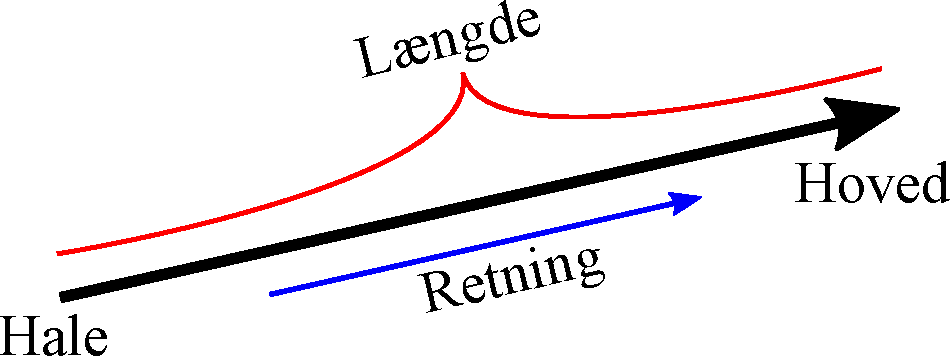
\includegraphics[scale=0.6]{matematik/fig/vektor.pdf}
	\caption{Den sorte pil er vektoren, og der er indikeret både vektorens længde og retning. }
	\label{vektorfig}
\end{figure}

Typisk vil man dog gerne regne med vektorer, og selvom det godt kan gøres vha. en grafisk metode, er der en anden repræsentation af vektorer, som egner sig bedre til dette. Denne kaldes for \emph{komposantform} (eller matrixform)  og tager udgangspunkt i et koordinatsystem. Da man i fysikken arbejder med den virkelige verden, som jo har tre rumlige dimensioner, vil vi i resten af afsnittet bruge et 3-dimensionalt koordinatsytem, som vist på Figur \ref{koordsys}. Specielt bruges et højrehåndet koordinatsystem, hvilket betyder, at hvis man tager højre hånd og peger sin tommelfinger i $x$-retningen og sin pegefinger i $y$-retningen, så vil langefingeren vise $z$-retningen, som det også ses på Figur \ref{koordsys}.\\
Ideen med komposantformen er, at man i et koordinatsystem kan beskrive en vektor, $\v{v}$, ved at angive tre tal $v_x,  v_y,  v_z$, som angiver, hvor meget vektoren peger i hhv. $x$-, $y$-, og $z$-retningen. Disse tal kaldes for vektorens komposanter, og man skriver vektoren:

\begin{equation}
\v{v} = \xyz{v_x}{v_y}{v_z}
\end{equation}

\vspace{2mm}

For at finde længden af vektoren, som man skriver $\abs{\v{v}}$, på komposantform, bruges Pythagoras sætning i tre dimensioner. Man får altså at:

\begin{equation}
\abs{\v{v}} = \sqrt{v_x^2 + v_y^2 + v_z^2}
\label{length}
\end{equation} 

\vspace{2mm}

Til sidst er det også vigtigt at vide, hvornår to vektorer er lig med hinanden. Det er de, hvis de har både samme længde og samme retning. På komposantform kan dette skrives:

\begin{equation}
\v{v} = \v{u} \quad \quad \text{hvis} \quad \quad
\begin{matrix}
v_x = u_x \\
v_y = u_y \\
v_z = u_z \\
\end{matrix}
\end{equation}

\vspace{2mm}

To vektorer er altså lig med hinanden, hvis deres komposanter er ens.\\

\begin{figure}[h!]
	\centering
	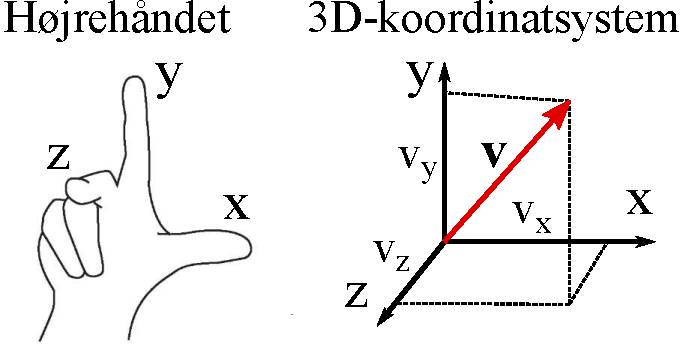
\includegraphics[scale=0.9]{matematik/fig/koordsys}
	\caption{På billedet til venstre ses reglen for et højrehåndet koordinatsystem. På billedet til højre er der vist et højrehåndet 3-dimensionalt koordinatsystem, og der er også indtegnet en vektor, $\v{v}$, med sine tre komposanter $v_x,  v_y,  v_z$.}
	\label{koordsys}
\end{figure}

\noindent
\textbf{Regneregler for Vektorer}\\

I dette afsnit skal vi se på, hvordan man regner med vektorer. Det første spørgsmål som man kunne stille sig selv i denne forbindelse er, om man kan lægge/trække vektorer til/fra hinanden. Det kan man godt, og det gøres ved at lægge/trække komposanterne til/fra hinanden i par. Det skrives:

\begin{equation}
\v{v} \pm \v{u} = \xyz{v_x}{v_y}{v_z} \pm \xyz{u_x}{u_y}{u_z} = \xyz{v_x \pm u_x}{v_y \pm u_y}{v_z \pm u_z}
\end{equation}
\vspace{2mm}

En anden ting som man kan gøre med en vektor, er at gange den med en konstant $a$. Det gøres ved at gange tallet på hver af komposanterne, altså:

\begin{equation}
a \cdot \v{v} = a \cdot \xyz{v_x}{v_y}{v_z} = \xyz{a \cdot v_x}{a \cdot v_y}{a \cdot v_z}
\end{equation}

\vspace{2mm}

Det næste naturlige spørgsmål er nu, om man kan gange og dividere vektorer med hinanden. Det viser sig at division af vektorer ikke er defineret, men at der til gengæld er to forskellige måder at gange vektorer sammen på, som begge kaldes for vektorprodukter.\\

Den første er \emph{skalarproduktet} (eller prikproduktet) og kaldes sådan, fordi resultatet er en skalar (altså et tal). Skalarproduktet af to vektorer skrives $\v{v} \cdot \v{u}$ og er defineret som:

\begin{equation}
\v{v} \cdot \v{u} = \xyz{v_x}{v_y}{v_z} \cdot \xyz{u_x}{u_y}{u_z}
= v_x \cdot u_x + v_y \cdot u_y + v_z \cdot u_z
\end{equation} 

\vspace{2mm}

Man tager altså vektorenes komposanter, ganger dem sammen i par og lægger det hele sammen. Specielt kan man kigge på skalarproduktet af en vektor med sig selv, og hvis man sammenligner med udtrykket for længden af en vektor, ligning \eqref{length}, ses, at $\v{v} \cdot \v{v} = \left| \v{v} \right|^2$. Det giver os en alternativ definition på længden af en vektor; $\abs{\v{v}} = \sqrt{\v{v} \cdot \v{v}}$.\\ 
Skalarproduktet har dog også en mere geometrisk definition, som tager udgangspunkt i vektorenes længde og vinklen mellem dem. Det er her vigtigt at understrege, at når man taler om vinklen mellem to vektorer, så menes der den mindste vinkel mellem dem, når man placerer halerne af vektorene oveni hinanden, som det ses på Figur \ref{dot_cross}. Med denne definition er skalarproduktet:

\begin{equation}
\v{v} \cdot \v{u} = \abs{\v{v}} \cdot \abs{\v{u}} \cdot \cos \theta
\end{equation} 


\vspace{2mm}

Det andet af de to vektorprodukter er \emph{krydsproduktet}, hvor resultatet er en ny vektor. Krydsproduktet skrives $\v{v} \times \v{u}$ og er defineret:

\begin{equation}
\v{v} \times \v{u} = \xyz{v_x}{v_y}{v_z} \times \xyz{u_x}{u_y}{u_z} = \xyz{v_y \cdot u_z - v_z \cdot u_y}{v_z \cdot u_x - v_x \cdot u_z}{v_x \cdot u_y - v_y \cdot u_x}
\end{equation} 

\vspace{2mm}

En vigtig egenskab ved krydsproduktet, som man ikke sådan lige kan se ud af definitionen er, at den resulterende vektor, $\v{c} = \v{v} \times \v{u}$, er vinkelret på både $\v{v}$ og på $\v{u}$. Kigger man igen på Figur \ref{dot_cross}, kan man da se, at der er to muligheder for, hvilken vej vektoren $\v{c}$ kan pege, så den er vinkelret på $\v{v}$ og $\v{u}$; nemlig ind i eller ud af figuren. Der er selvfølgelig kun en af disse, som er den rigtige retning, og heldigvis er der en nem huskeregel (typisk kaldet højrehåndsreglen) til at finde den rigtige. Man tager højre hånd og peger tommelfingeren i retningen af den første vektor og peger så sin pegefinger i retningen af den anden vektor. Da vil langefingeren give retningen af den nye vektor, $\v{c}$, på samme måde som den angiver $z$-retningen i et højrehåndet koordinatsystem. Tager man eksemplet på Figur \ref{dot_cross}, vil $\v{c}$ pege ind i figuren.\\
Ligesom med skalarproduktet har krydsproduktet også en mere geometrisk fortolkning. Det gælder nemlig at størrelsen af den vektor, som man får, når man laver et krydsprodukt, kan udtrykkes vha. længden af de to vektorer som man krydser med hinanden og vinklen mellem dem. Der gælder:

\begin{equation}
\abs{\v{v} \times \v{u}} = \abs{\v{v}} \cdot \abs{\v{u}} \cdot \sin \theta 
\end{equation}

\vspace{2mm}

\begin{figure}[h!]
	\centering
	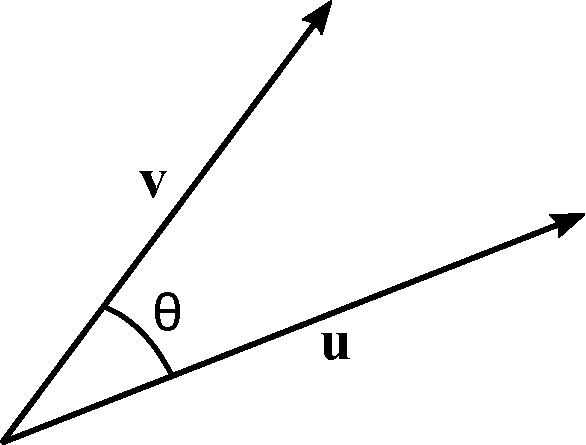
\includegraphics[scale=0.7]{matematik/fig/dot_cross.pdf}
	\caption{To vektorer og deres mellemliggende vinkel.}
	\label{dot_cross}
\end{figure}

Det sidste begreb er \emph{enhedsvektorer}, der er vektorer, som har en længde på 1. For at kunne kende forskel på en almindelig vektor og en enhedsvektor, bruger man en speciel notation, hvor man sætter en "hat" over vektoren, $\hatvec{v}$. Enhedsvektorer opfylder de samme regneregler som almindelige vektorer, og på den måde er der ikke meget nyt i dem. De er dog et vigtigt notationsmæssigt redskab og bruges i mange dele af fysikken. Specielt bruger man ofte enhedsvektorer, der peger langs en af de tre koordinatakser. Disse har en speciel notation og er skrevet op nedenfor:

\begin{equation}
\xhat = \xyz{1}{0}{0} \ , \quad \quad \yhat = \xyz{0}{1}{0} \ , \quad \quad \zhat = \xyz{0}{0}{1}
\end{equation}

\vspace{2mm}

Med disse tre enhedsvektorer kan man nu skrive enhver vektor, $\v{v}$, på følgende måde:

$$\v{v} = \xyz{v_x}{v_y}{v_z} = \xyz{v_x}{0}{0} + \xyz{0}{v_y}{0} + \xyz{0}{0}{v_z} = v_x \xhat + v_y \yhat + v_z \zhat$$

\vspace{2mm}

Denne metode, hvor man skriver en vektor som summen af flere andre vektorer, er vigtig at bide mærke i. Hvis en vektor, $\v{v}$, repræsenterer en fysisk størrelse, f.eks. en kraft, så vil den fysiske størrelse være uændret, om man skriver vektoren på den ene eller anden måde. Dette er praktisk, da man selv kan vælge på hvilken måde man skriver vektoren, alt efter hvilken fysisk problemstilling man prøver at løse. 


\section{Vektorfelter}

I dette afsnit skal vi kigge på vektorfelter, som er et meget udbredt værktøj indenfor fysikken. For at kunne give en ordentlig forklaring af, hvad et vektorfelt er, er det nyttigt først at kigge på funktioner af to eller tre variable. Når man arbejder med to variable, bruger man typisk $x$ og $y$, og man skriver en funktion $f(x,y)$ for at vise, at funktionen afhænger både af værdien af $x$ og af værdien af $y$. Funktionen $f(x,y)$ tager altså ethvert punkt $(x',y')$ i $xy$-planen og giver punktet en bestemt værdi; nemlig $f(x',y')$. Et godt eksempel på en funktion af to variable kunne f.eks. være højden over havet i Danmark, som afhænger af, både hvor langt nord/syd på og øst/vest på man befinder sig. På helt samme måde kan man arbejde med funktioner af tre variable, typisk $x,y,z$, og man skriver en funktion $f(x,y,z)$. Her tager funktionen $f(x,y,z)$ ethvert punkt $(x',y',z')$ i et 3-dimensionalt koordinatsystem og giver igen punktet en bestemt værdi; nemlig $f(x',y',z')$. Et godt eksempel på en funktion af tre variable er temperaturen i et rum, som jo kan ændre sig både hvis man går frem og tilbage, hvis man går til siderne eller hvis man bevæger sig op og ned.\\
Med denne introduktion er vi nu klar til at kigge på vektorfelter, og for at gøre det nemmere at illustrere nogle af de vigtige begreber, starter vi med kun at arbejde i to dimensioner, og holder os derfor til $xy$-planen.\\

Et vektorfelt i to dimensioner, som skrives $\v{F}(x,y)$, er på mange måder ligesom en funktion af to variable. Der er dog den forskel, at hvor en funktion, $f(x,y)$, tager alle punkter i $xy$-planen og giver dem en bestemt værdi (altså et tal), så tager et vektorfelt, $\v{F}(x,y)$, alle punkter i $xy$-planen og giver dem hver en bestemt vektor. Dette kan være en lidt speciel ide første gang man møder den, og derfor er der plottet et eksempel i Figur \ref{vecfield}. Når man plotter et vektorfelt tegner man ikke vektorerne i alle punkter, da man så ikke vil kunne se noget for alle de vektorer, der vil ligge oveni hinanden. I stedet plotter man blot nogle enkelte af vektorene for at få en generel ide om, hvordan vektorfeltet ser ud.

\begin{figure}[h!]
	\centering
	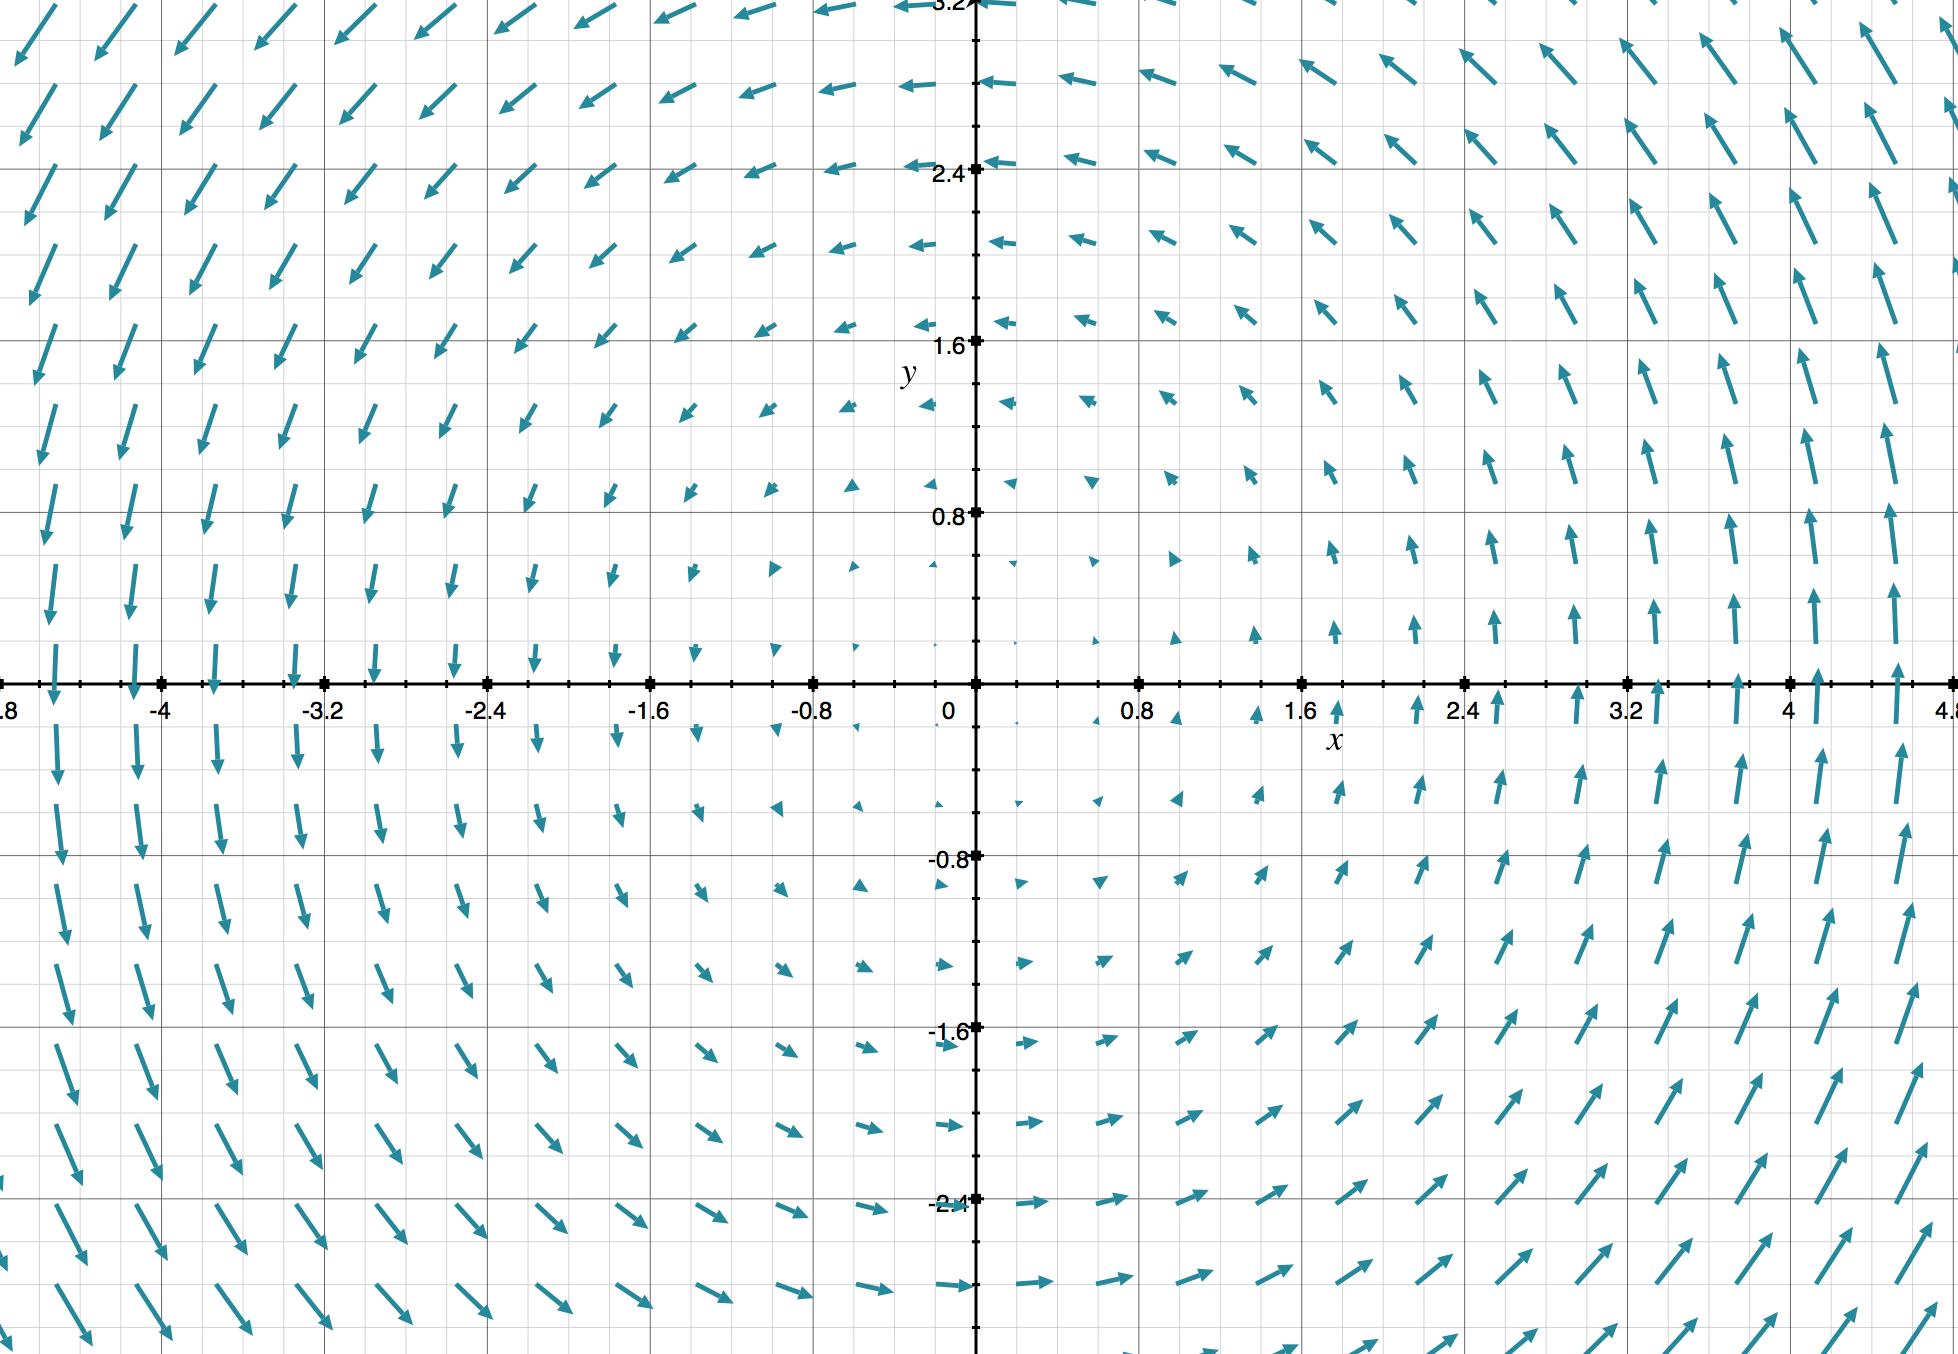
\includegraphics[scale=0.38]{matematik/fig/vecfield_2D.png}
	\caption{På figuren ses et eksempel på et vektorfelt i to dimensioner. Det kunne f.eks. være et vektorfelt, der beskriver vand, der hvirvler rundet om centrum, og hver af vektorene ville da angive vandets hastighed i det punkt, hvor vektorens hale ligger.}
	\label{vecfield}
\end{figure}

Ligesom med en normal vektor, så viser komposantformen sig, at være den bedste måde at arbejde med vektorfelter på. Givet et vektorfelt, $\v{F}(x,y)$, kan man altså skrive det vha. en $x$ og $y$ komposant, $F_x (x,y)$ og $F_y(x,y)$, der begge er funktioner af to variable. Man kan altså skrive et vektorfelt i to dimensioner:

\begin{equation}
\v{F} (x,y) = \xy{F_x(x,y)}{F_y(x,y)} = \xy{F_x}{F_y}
\end{equation}

\vspace{2mm}

Vektorfelter i tre dimensioner, som skrives $\v{F}(x,y,z)$, fungerer på samme måde som i to dimensioner og tager altså ethvert punkt i et 3-dimensionalt koordinatsystem og giver punktet en bestemt vektor. Igen kan man skrive vektorfeltet på komposantform, hvor der her er både en $x$, $y$ og $z$ komposant, $F_x (x,y,z)$, $F_y (x,y,z)$ og $F_z (x,y,z)$. Man kan altså skrive vektorfelter i tre dimensioner som følger

\begin{equation}
\v{F}(x,y,z) = \xyz{F_x(x,y,z)}{F_y(x,y,z)}{F_z(x,y,z)} = \xyz{F_x}{F_y}{F_z} =  F_x \xhat + F_y \yhat + F_z \zhat \ ,
\end{equation} 

\vspace{2mm}

hvor den sidste måde at skrive vektorfeltet på bruger de tre enhedsvektorer, $\xhat$, $\yhat$, $\zhat$, reglen for hvordan man ganger et tal (eller en funktion) med en vektor  og måden man ligger vektorer sammen på. Det gælder nemlig, at alle de regneregler som er blevet gennemgået for vektorer i tre dimensioner i vektorafsnittet, også gælder for vektorfelter i tre dimensioner.\\

\noindent
\textbf{Differentiering af Vektorfelter}\\

Ligesom differentialregningen er et vigtigt redskab, når man arbejder med funktioner, så er den også vigtig i forhold til vektorfelter. Før vi kan kigge på, hvordan man differentierer vektorfelter, og hvad det egentligt betyder, er der et vigtigt begreb kaldet partiel differentiation, som skal på plads først.\\

Når man differentierer funktioner med mere end en variabel er den letteste metode partiel differentiation. Her differentierer man funktionen i forhold til én variabel, og fastholder alle de andre, hvilket vil sige, at man behandler dem, som var de konstanter. Partiel differentiation minder derfor meget om enkeltvariabel differentiation. Funktionen $f(x,y,z)=xyz$ differentieres således partielt:

$$\frac{\partial f}{\partial x} = yz ~~,~~ \frac{\partial f}{\partial y} = xz ~~ \text{og} ~~  \frac{\partial f}{\partial z} = xy$$

\vspace{2mm}

Videre er vi også nødt til at indføre en differentialoperator. Generelt set er en operator noget som "opererer" (gør noget bestemt) ved f.eks. en funktion eller vektor. En differentialoperator er altså en operator som går ind og laver en differentialoperation på en funktion eller vektor. Her skal vi specielt kigge på differentialoperatoren kaldet nabla (eller del), som har en speciel notation, $\gv{\nabla}$. Nablaoperatoren skrives:

\begin{equation}
\gv{\nabla} = \xyz{\partial / \partial x}{\partial / \partial y}{\partial / \partial z}
\end{equation}

\vspace{2mm}

Som man kan se ligner nabla en vektor, men man skal huske på, at det er en operator, og at den derfor ikke kan behandles fuldstændigt som en vektor. F.eks. giver det ikke meningen, at snakke om længden af nabla, som man kan gøre med en vektor. For at give en bedre ide om, hvordan en differentialoperator virker, vil vi kigge på, hvad der sker, hvis man lader nabla virke på en funktion. Givet en funktion, $f(x,y,z)$, virker nabla på den således:

\begin{equation}
\gv{\nabla} f = \xyz{\partial / \partial x}{\partial / \partial y}{\partial / \partial z} f = \xyz{\partial f / \partial x}{\partial f / \partial y}{\partial f / \partial z}
\end{equation}

\vspace{2mm}

Udtrykket, $\gv{\nabla}f$, kaldes for \emph{gradienten} af funktionen, og det ses, at når man lader nabla operere på en funktion, får man et vektorfelt som resultatet. Gradienten er et helt specielt vektorfelt, der giver os information omkring, hvordan funktionen, $f$, ændre sig i rummet. I ethvert punkt, $\left( x,y,z \right)$, vil gradienten nemlig pege i den retning, hvor funktionen ændre sig hurtigst. Hvis f.eks. en funktion, $f$, angiver temperaturen i et rum, så vil $\grad{f}$ til ethvert punkt i rummet fortælle os, i hvilken retning man vil opleve den største temperaturstigning, hvis man bevæger sig en infinitesimal længde væk fra det punkt man kigger på.\\

Nu hvor vi har kigget både på partiel differentiation og differentialoperatoren nabla, er vi klar til at introducere, hvordan man differentierer et vektorfelt. Det kan gøres på to forskellige måder, og begge tager udgangspunkt i nabla.\\

Den første måde at differentiere et vektorfelt på kaldes for \emph{divergensen}, og man kan tænke på den som et prikprodukt mellem nabla og et vektorfelt. Divergensen af et vektorfelt skrives:

\begin{equation}
\div{\v{F}} = \xyz{\partial  / \partial x}{\partial  / \partial y}{\partial  / \partial z} \cdot \xyz{F_x}{F_y}{F_z}  = \frac{\partial F_x}{\partial x}+\frac{\partial F_y}{\partial y}+\frac{\partial F_z}{\partial z}
\end{equation}

\vspace{2mm}

Kigger man nærmere på divergensen i et enkelt punkt, vil denne angive, hvor meget vektorfeltet "udstråler" fra punktet. Hvis et vektorfelt, $\v{F}$, f.eks. angiver hastighed af partiklerne i en væske, vil divergensen af vektorfeltet, $\div{F}$, i et punkt, fortælle hvor meget væske der samlet set strømmer ud fra dette punkt. En positiv divergens i et punkt fortæller således i dette eksempel, at der strømmer mere væske væk fra end til punktet, mens en negativ divergens i et punkt fortæller, at der strømmer mere væske til punktet end væk fra det.\\

Den anden måde at differentiere et vektorfelt på kaldes for \emph{rotationen} (også kaldet curl), og man kan tænke på den som et krydsprodukt mellem nabla og et vektorfelt. Rotationen af et vektorfelt skrives:

\begin{equation}
\curl{\v{F}} = \xyz{\partial  / \partial x}{\partial  / \partial y}{\partial  / \partial z} \times \xyz{F_x}{F_y}{F_z} = \xyz{\partial F_z/\partial y - \partial F_y/\partial z}{\partial F_x/\partial z - \partial F_z/\partial x}{\partial F_y/\partial x - \partial F_x/\partial y} 
\end{equation}

\vspace{2mm}

Kigger man også her nærmere på rotationen i et punkt, giver den et mål for, hvor meget vektorfeltet "hvirvler" omkring dette punkt. Igen kan man bruge eksemplet, hvor et vektorfelt, $\v{F}$, angiver hastigheden af partiklerne i en væske. Vi kan nu forestille os, at vi tager et lille støvfnug og sænker det ned i væsken. Rotationen i det punkt hvor støvfnugget befinder sig, vil da fortælle os om, hvor stor en tendens væsken har til at få støvfnugget til at rotere omkring sig selv i dette punkt, og hvilken akse det vil rotere omkring.\\

\begin{figure}[h!]
\centering
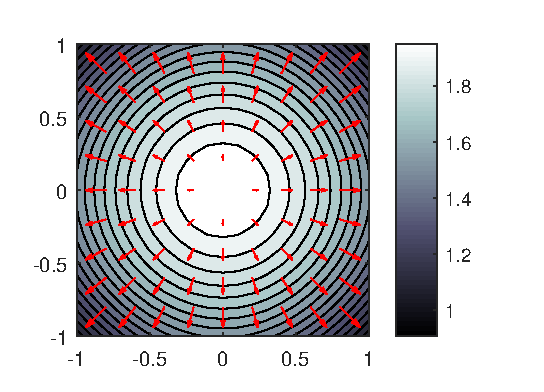
\includegraphics[width = 0.45\textwidth]{matematik/fig/div.eps}
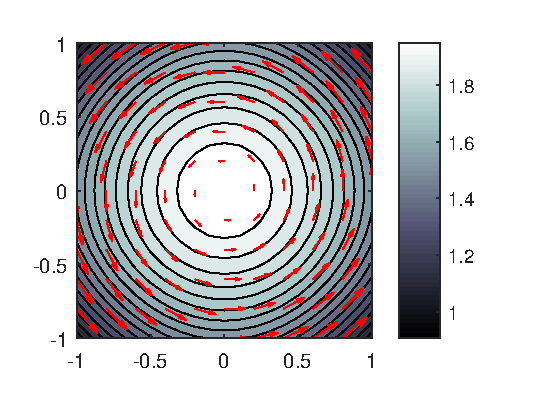
\includegraphics[width = 0.45\textwidth]{matematik/fig/rot.eps}
\caption{To vektorfelter, til venstre er divergensen plottet med kontourplottet, til højre er det rotationen. Funktionerne er valgt så den af operationerne der ikke er vist er lig nul. Funktionerne er $\v{f}(x,y) = \sin(x)\xhat+\sin(y)\yhat$ og $\v{g}(x) = -sin(y)\xhat-\sin(x)\yhat$. De har $\v \nabla \cdot \v{f} = \cos(x)+\cos(y)$ og $\v\nabla\times \v{g}=(\cos(x)+\cos(y))\zhat$.}
\end{figure}

Nu hvor vi har kigget på både divergensen og rotationen, er det på sin plads hurtigt at nævne, hvorfor disse begreber er vigtige, når man arbejder med vektorfelter. Det første svar på dette spørgsmål er, at divergensen og rotationen, som gennemgået ovenfor, hjælper os med at beskrive, hvordan vektorfelter opfører sig. Det andet (og på mange måder vigtigere) svar er, at for "pæne" vektorfelter\footnote{Med pæne menes, at de opfylder nogle bestemt matematiske betingelser. Vi vil dog ikke kigge nærmere på hvilke specifikke betingelser det er, eller hvorfor det netop er disse betingelser, der er nødvendige.}, $\v{F}$, som er den eneste type i vil møde på campen, kan man beskrive vektorfeltet til fulde, hvis blot man kender divergens, $\div{\v{F}}$, og rotationen, $\curl{\v{F}}$, af vektorfeltet. Da man i fysiske problemstillinger ofte vil kende disse men ikke vektorfeltet selv, og da divergensen og rotationen typisk er nemmere at arbejde med en vektorfeltet, $\v{F}$, er dette resultat utroligt vigtigt.


\section{Matricer og Lineære Transformationer}

En lineær transformation er en funktion, der opfylder to krav. At summen af to vektorer transformeret, er lig summen af de to vektorer transformerets sum.
Lineære transformationer tager en vektor som indput, og giver en ny vektor som output. Tænk på tranformationen som $f$ i $f(x)$ og vektoren som $x$.
\begin{equation}
T(\v v+\v u) = T(\v v) + T(\v u)
\end{equation}
Det andet krav er at det samme gælder når man ganger med et tal.
\begin{equation}
T(a\v v) = aT(\v v)
\end{equation}
I en dimension er funktioner af formen $f(x) = ax$ den eneste type hvor det gælder, derfor navnet lineær.

Siden en vektor altid kan beskrives som en sum af vores enhedsvektorer, er det kun nødvendigt at vide hvordan de transformerer for at vide hvordan alle vektorer transformerer. En simpel lineær transformation i $xy$-planen er spejling i $x$ aksen. Her er $\xhat$ uændret og $\yhat$ skrifter fortegn.
\begin{align}
S_x(\xhat) &= \xhat\\
S_x(\yhat) &= -\yhat
\end{align}
Med denne viden er det muligt at spejle en hver vektor i $x$-aksen:
\begin{equation}
S(\v v) = S(v_x\xhat+v_y\yhat) = v_xS(\xhat)+v_yS(\yhat) = v_x\xhat-v_y\yhat = \xy{v_x}{-v_y}
\end{equation}
Dette er en mulig måde at gøre det på, men det bliver hurtigt grimt for bare lidt mere komplicerede udregninger. Istedet beskrives lineære transformationer oftest med matricer. Lige som en vektor kan skrives som en søjle af tal kan en matrix skrives som et rektangulært skema. Matricer kan have vilkårlig størelse, men vi vil primært beskæftige os med $2\times 2$ matricer.
Ser man transformationen som $f$ i $f(x)$ vil matricen svare til ligningen der beskriver funktionen.

\begin{equation}
\v A= \begin{bmatrix}
a & b\\c&d
\end{bmatrix}
\end{equation}

Matricer lægges sammen og ganges med tal indgangsvist, lige som vektorer.
\begin{align}
\v A_1+\v A_2 &= \begin{bmatrix}
a_1+a_2&b_1+b_2\\c_1+c_2&d_1+d_2
\end{bmatrix}\\
\alpha \v A &= \begin{bmatrix}
\alpha a & \alpha b\\
\alpha c & \alpha d
\end{bmatrix}
\end{align} 

Man kan gange en matrix på en vektor hvilket giver en ny vektor, så længe matricen er lige så bred som vektoren er høj. Man finder den resulterende vektor ved at lægge alle indgangene i den oprindelige vektor ganget med en indgang i den tilsvarende række(vandret) af matricen. 
\begin{equation}
\begin{bmatrix}
a&b\\c&d
\end{bmatrix}
\xy{v_x}{v_y} = \xy{av_x+bv_y}{cv_x+dv_y}
\end{equation}
Bemærk at hvis man ganger en matrix på vektorer som $\begin{bsmallmatrix}1\\0\end{bsmallmatrix}$ og $\begin{bsmallmatrix}0\\1\end{bsmallmatrix}$ vil den resulterende vektor være henholdvis første eller anden søjle(lodret) af matricen. Inspireret af dette kan spejlingen fra før beskrives men en matrix, og transformationen udregnes med et matrixprodukt.
\begin{equation}
S(\v v)=\v S \v v = \begin{bmatrix}
1 & 0\\
0 & -1
\end{bmatrix}
\xy{v_x}{-v_y} = \xy{v_x}{-v_y}
\end{equation}

Matricer kan også ganges med hinanden, dette gøres ved at gange den venstre matrix på hver søjle af den højre matrix som var de enkelte vektorer.
\begin{equation}
\v A_1 \v A_2 = 
\begin{bmatrix}
a_1&b_1\\c_1&d_1
\end{bmatrix}
\begin{bmatrix}
a_2&b_2\\c_2&d_2
\end{bmatrix}
=
\begin{bmatrix}
a_1a_2+b_1c_2&a_1b_2+b_1d_2\\
c_1a_2+d_1c_2&c_1b_2+d_1d_2
\end{bmatrix}
\end{equation}

Bemærk at hvis man byttede om på $a$'erne og $b$'erne ville resultatet ikke blive det samme. Det betyder at rækkefølgen af matricerne er afgørende for resultatet. Matricer ganges på fra venstre, så matricen længst til højre svarer til den transformation der udføres først.
En vigtig matrix er identitetsmatricen $\v I= \begin{bsmallmatrix}1 & 0\\0& 1\end{bsmallmatrix}$. Den svarer til tallet 1, på den måde at ganger man noget med $\v{I}$ vil det være uændret. 


%\section{Taylor-approksimation}

%I fysik ender man ofte med nogle differentialligninger, som man ikke
%kender eksakte løsninger til. Derfor er man ofte nød til at
%simplificere tingene lidt ved at lave nogle approksimationer, der er
%passende for det fysiske system, man kigger på. Hvis man kigger på
%svingninger af et pendul, er det måske rimeligt at antage, at
%svingningerne er små, hvilket kan simplificere ens ligningerne
%betydeligt.

%Lad $f$ være en funktion af $x$ og evt. flere variable. Muligvis er
%$f(x)$ en kompliceret funktion, men vi er kun interesseret i, hvordan
%$f(x)$ ser ud omkring et bestemt punkt, lad os sige $x_0$. Vi er derfor
%tilfredse, hvis vi har et approksimativt udtryk for $f(x)$, når
%$x \approx x_0$. Et sådant approksimativt udtryk er
%Taylor-approksimationen for $f(x)$ omkring punktet $x_0$.

%\begin{enumerate}[resume]
%\item\label{itm:d-taylor} \textbf{Taylor-approksimation til anden orden.}\\
%  Når $x \approx x_0$ er funktionen $f(x)$ approksimativt givet ved
%  \[
%  f(x) \approx f(x_0) + (x-x_0) \, [\d{f}{x}]_{x=x_0}
%  + \tfrac{1}{2} (x-x_0)^2 \, [\dd{f}{x}]_{x=x_0} \; .
%  \]
%  Her skal $[\d{f}{x}]_{x=x_0}$ forstås som at man beregner
%  $\d{f}{x}$, som er en funktion af $x$, og dernæst sætter $x=x_0$, så
%  vi får hældningen i punktet $x_0$. Tilsvarende er
%  $[\dd{f}{x}]_{x=x_0}$ den dobbelte differentierede, $\dd{f}{x}$, med
%  $x=x_0$, så vi får hældningen af hældningen i $x_0$. Dette betyder,
%  at Taylor-approksimationen ovenfor er en parabel.
%\end{enumerate}
%Lad os retfærdigøre Taylor-approksimationen via et eksempel. Lad os
%approksimere funktionen $f(x) = 1 + x^2 + \tfrac{1}{3} x^3$ omkring
%det lokale minimum i punktet $0$ (dvs. vi sætter $x_0 = 0$), se
%tegningen til venstre. Vi betragter leddene i approksimationen ét
%efter ét, og approksimationen bliver bedre jo flere led, vi
%medtager.

%\begin{center}
%  \begin{tikzpicture}
%    \begin{scope}[shift={(0,0)}]
%      \draw [->] (-2.2,0) -- (2.2,0);
%      \node [right] at (2.2,0) {$x$};
%      \draw [->] (0,-.1) -- (0,3.3);
%      \node [above] at (0,3.3) {$f(x)$};
%      \draw (-.1,1) -- (.1,1);
%      \node [left] at (-.1,1) {$1$};
%      \node [below] at (0,-.1) {$0$};
%      \draw (-1,-.1) -- (-1,.1);
%      \node [below] at (-1,-.1) {$-1$};
%      \draw (1,-.1) -- (1,.1);
%      \node [below] at (1,-.1) {$1$};
%      \draw [blue, domain=-2.2:1.2, samples=300]
%      plot (\x, {1 + \x*\x + 1/3*\x*\x*\x});
%    \end{scope}
%    % 
%    \begin{scope}[shift={(8,0)}]
%      \draw [->] (-2.2,0) -- (2.2,0);
%      \node [right] at (2.2,0) {$x$};
%      \draw [->] (0,-.1) -- (0,3.3);
%      \node [above] at (0,3.3) {$f(x)$};
%      \draw (-.1,1) -- (.1,1);
%      \node [left] at (-.1,1) {$1$};
%      \node [below] at (0,-.1) {$0$};
%      \draw (-1,-.1) -- (-1,.1);
%      \node [below] at (-1,-.1) {$-1$};
%      \draw (1,-.1) -- (1,.1);
%      \node [below] at (1,-.1) {$1$};
%      \draw [blue, domain=-2.2:1.2, samples=300]
%      plot (\x, {1 + \x*\x + 1/3*\x*\x*\x});
%      \draw [green, domain=-2.2:2.2, samples=300]
%      plot (\x, {1});
%      \draw [red, domain=-1.4:1.4, samples=300]
%      plot (\x, {1 + \x*\x});
%    \end{scope}
%  \end{tikzpicture}
%\end{center}

%Det første led er konstant funktionsværdien i punktet $x_0$, hvilket
%er en grov approksimation. I vores tilfælde er $f(x_0) = f(0) = 1$,
%hvilket er den grønne linje på tegningen til højre.

%Det næste led, $(x-x_0) \, [\d{f}{x}]_ {x=x_0}$, er en lineær funktion
%med samme hældning som funktionen i $x_0$. Medtages dette
%led, vil vi generelt få en lidt bedre approksimation. I vores tilfælde
%er $\d{f}{x} = 2x + x^2$, hvilket i punktet $0$ tager værdien
%$[\d{f}{x}]_{x=0} = [2x + x^2]_{x=0} = 0$, så det lineære led i
%approksimationen bidrager ikke.

%Det næste led, $\tfrac{1}{2} (x-x_0)^2 \, [\dd{f}{x}]_ {x=x_0}$, er en
%parabel med samme krumning som funktionen i $x_0$. I vores tilfælde er
%$\dd{f}{x} = 2 + 2x$, så $[\dd{f}{x}]_ {x=x_0} = [2 + 2x]_{x=0} =
%2$. Dermed bliver Taylor-approksimationen
%\[
%f(x) \approx 1 + x^2 \qquad \text{når } x \approx 0 \; ,
%\]
%hvilket er den røde linje på tegningen. Som det ses er dette en
%udmærket approksimation af den blå linje, men kun så længe $x \approx
%0$. Hvis vi vil approksimere funktionen omkring et andet punkt, skal
%vi lave en ny Taylor-approksimation med et andet $x_0$, og så vil vi
%få et andet udtryk end den ovenfor fundne.

%Approksimationen kan generelt forbedres ved at tage flere led med af
%typen $\tfrac{1}{n!} (x-x_0)^n \, [\partial^n_x f]_{x=x_0}$ for
%$n=3,4,\dots$, men dette er ikke nødvendigt for os, og vi er tilfredse
%med de tre første led.




%%% Local Variables: 
%%% mode: latex
%%% TeX-master: "../main"
%%% End: 
